\chapter{Recursive Algorithms}
\label{ch:recursive_algorithms}

The same equations can be expressed as a large joint-space calculation or as a sequence of local rigid-body balances. Recursion organizes that calculation around the connections between bodies. It lets us ask, in order, how motion reaches a segment and what wrench its motion requires from the rest of the mechanism. These are complementary questions: adding segment velocities without changing frames is wrong, and adding forces without shifting their moments is equally wrong.

For a golf model, this organization makes the physical dependencies inspectable. A hand changes the club's motion through an interface wrench; the equal and opposite wrench loads the arm. Ground forces enter through the feet. Joint torques are projections of transmitted wrenches onto allowed relative motions. Computing those quantities reliably is a prerequisite for studying coordination, power, constraints and delivery. It does not by itself establish which muscular strategy a golfer used, or which change would improve the next swing.

\section{What Is Being Computed?}
\label{sec:history_rnea}
\label{laymans:context_box}

We distinguish three operations. Forward kinematics maps joint configuration to body poses and, with joint rates, body velocities. Inverse dynamics maps prescribed motion and known external loads to the generalized forces required by a specified mechanical model. Forward dynamics maps applied forces and the current state to acceleration. A time integrator then advances the state; an inverse-dynamics evaluation alone does not simulate a swing.

For a fixed-base rigid tree with independent scalar joints, write
\begin{equation}
 M(q)\ddot q+h(q,\dot q)=\tau+\sum_i J_i(q)^T f_i^{\rm ext}.
 \label{eq:lagrange_matrix}
\end{equation}

Here $h$ includes velocity-product and gravitational terms; $f_i^{\rm ext}$ is a wrench applied to body $i$, and $J_i$ maps joint rates to that body's twist in the same frame and about the same origin as the wrench. Joint friction, springs and actuator dynamics must be specified separately. In particular, a computed net joint torque is not a uniquely identified muscle force.

Recursive Newton--Euler inverse dynamics (RNEA) evaluates the left-hand side and known-load subtraction without constructing $M$. Its arithmetic cost grows linearly with the number of bodies when joint dimensions and per-joint calculations are bounded. This is an algorithmic property of a tree, not a claim that Lagrangian mechanics becomes intractable beyond some number of joints. Factored expressions, automatic differentiation and numerical matrix methods also avoid enormous symbolic expansions. No universal control frequency follows from an asymptotic complexity class.

Luh, Walker and Paul's 1980 paper is an important historical reference for manipulator dynamics computation; Featherstone's spatial-vector treatment and Lynch and Park's geometric formulation provide systematic accounts of the algorithms~\cite{luh1980,Featherstone2008,Lynch2017}. The derivation below fixes its conventions explicitly because superficially similar published recursions can use opposite transform directions or external-force signs.

\section{A Tree and Its Traversal Order}
\label{sec:tree_structure}
\label{sec:branching_trees}

A kinematic tree is connected and has no cycles. Let body $0$ be a fixed base, and let bodies $1,\ldots,N$ each attach through one joint to a parent $\lambda(i)$. Choose any numbering with $\lambda(i)<i$. This ordering is not unique: siblings can be exchanged. It ensures that a parent's motion is available during an outward pass and that every child's accumulated wrench is available during a reverse pass. The inward pass therefore visits children before parents.

For example, $\lambda=(0,1,1,3)$ describes four moving bodies: body 1 attaches to the base, bodies 2 and 3 branch from body 1, and body 4 attaches to body 3. A list of parent indices is enough for the recursions; one can accumulate each child's contribution directly into its parent without searching the whole list for children. A three-body chain instead has $\lambda=(0,1,2)$. Adding a serial gripper joint at its end does not create a branch; two separate children attached to the same body do.

\begin{figure}[htbp]
\centering
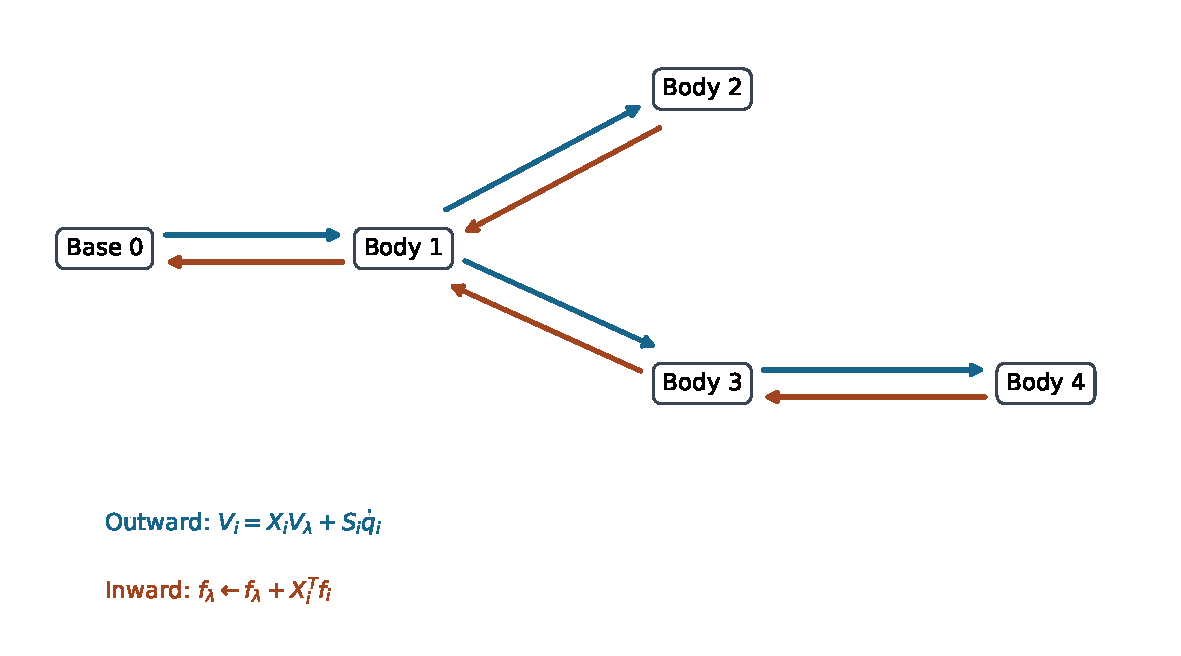
\includegraphics[width=\linewidth]{../figures/recursive_tree.pdf}
\caption{A Four-Body Tree With Parent Array (0, 1, 1, 3). Motion Propagates Outward; Subtree Wrenches Accumulate Inward.}
\label{fig:kinematic_tree}
\end{figure}

Each body frame is rigidly attached to that body. Its origin may be at a joint, the center of mass, or another fixed point, provided its inertia, joint subspace and loads all use that choice. The base is a boundary condition, not an extra actuated joint. A floating pelvis or a robot in flight requires a moving-base formulation. Treating a foot as a permanently welded base is a physical assumption with consequences for the reaction forces and allowed motion.

\section{Frame Changes and Their Power Dual}
\label{sec:adjoint}

Define $T_{AB}=(R,p)\in SE(3)$ by $x_A=Rx_B+p$: it maps point coordinates from frame $B$ to frame $A$. Thus $p$ locates the origin of $B$ in $A$. Use angular-first motion vectors $V=(\omega,v)$ and moment-first wrenches $f=(n,F)$. A rigid velocity field in $B$ has point velocity $u_B(x_B)=v_B+\omega_B\times x_B$. Reexpressing that same field in $A$ gives
\begin{equation}
 \begin{aligned}
 u_A(x_A)&=R v_B+(R\omega_B)\times(x_A-p),\\
 \omega_A&=R\omega_B,\qquad v_A=Rv_B+p\times R\omega_B.
 \end{aligned}
 \label{eq:adjoint_velocity}
\end{equation}

This is a coordinate change of the same physical motion field. If we instead compare the velocities of two bodies moving relative to each other, their relative twist must also be included.

With $[p]_\times a=p\times a$, the motion transform is
\begin{equation}
 X_{AB}=\operatorname{Ad}_{T_{AB}}
 =\begin{bmatrix}R&0\\{}[p]_\times R&R\end{bmatrix},\qquad
 X_{AB}^{-1}=\begin{bmatrix}R^T&0\\-R^T[p]_\times&R^T\end{bmatrix}.
 \label{eq:adjoint_matrix}
\end{equation}

Every rigid transform has an invertible adjoint. The matrix is generally not orthogonal: moving an origin mixes angular motion and linear velocity. Its numerical condition number depends on the origin and on the relative scaling of angular and translational units. This is different from loss of rank of a mechanism's task Jacobian.

\subsection{Wrenches Follow From Virtual Power}

Demand that $f_A^T V_A=f_B^T V_B$ for every twist. Since $V_A=X_{AB}V_B$, the two equivalent force relations are
\begin{equation}
 f_A=X_{AB}^{-T}f_B
 =\begin{bmatrix}R&[p]_\times R\\0&R\end{bmatrix}f_B,
 \qquad f_B=X_{AB}^{T}f_A.
 \label{eq:adjoint_force}
\end{equation}

The force rotates as $F_A=RF_B$; the moment also acquires the lever arm $p\times RF_B$. For a child-motion transform $X_i$ that maps parent coordinates into child coordinates, the child's wrench returns to the parent as $X_i^T f_i$. The inverse transpose maps a wrench in the same direction as the motion-coordinate change; the transpose maps it in the reverse direction. Keeping the direction explicit prevents a common sign and lever-arm error.

A force sensor reporting a force at a hand or clubhead must be converted to a wrench about the chosen body origin. If a force $F$ acts at body-coordinate point $r$ with applied couple $n_0$, then $f=(n_0+r\times F,F)$. Merely rotating the measured force leaves out its moment. The identity $f^T J\dot q=(J^Tf)^T\dot q$ then explains the generalized-load mapping in the equations of motion.

\section{Recursive Forward Kinematics}
\label{sec:forward_kinematics}
\index{Kinematics}
\label{laymans:recursive_intuition}

Let $T_{i\lambda}$ map parent coordinates to body $i$, and set $X_i=\operatorname{Ad}_{T_{i\lambda}}$. A joint model supplies this relative transform at $q_i$ and a local motion subspace $S_i$. For an ideal revolute joint through the child-frame origin about its unit $z$ axis, $S_i=(0,0,1,0,0,0)^T$; for translation along local $x$, $S_i=(0,0,0,1,0,0)^T$. An offset rotation axis has a nonzero linear part. Revolute and prismatic coordinates have different units, so their generalized forces are torques and forces respectively.

Absolute poses and body velocities propagate as
\begin{equation}
 T_{Wi}=T_{W\lambda(i)}T_{i\lambda}^{-1},\qquad
 V_i=X_iV_{\lambda(i)}+V_{Ji},\qquad V_{Ji}=S_i\dot q_i.
 \label{eq:velocity_recursion}
\end{equation}

The inverse in the pose equation follows from our declared direction; using the same local matrix without inversion would describe a different mapping. Relative transforms suffice for RNEA. Absolute poses are useful for visualization, world-frame loads and contact geometry, but need not be reconstructed during every force accumulation.

At a body-fixed point $r$, the body's local Cartesian velocity is $v_i+\omega_i\times r$. Rotate this vector into world coordinates for a clubhead-speed calculation. Segment angular speeds alone omit both origin motion and the point's lever arm. Adding speeds as scalar magnitudes also discards directions and can turn cancellation into apparent amplification.

\subsection{Exponentials and Numerical Representation}

For fixed space screws $\xi_j$, a serial-chain body pose has the product-of-exponentials form $T_{Wi}(q)=\exp(\widehat\xi_1q_1)\cdots\exp(\widehat\xi_iq_i)M_i$, with its own home pose $M_i$. Partial exponential products without those home poses are not generally the physical link poses. Body screws, space screws and relative joint transforms are interchangeable only through the appropriate coordinate conversions.

Pure translation is regular: if $\widehat\xi=\left[\begin{smallmatrix}0&v\\0&0\end{smallmatrix}\right]$, then $\widehat\xi^2=0$ and $\exp(q\widehat\xi)=I+q\widehat\xi$. There is no rank test or pseudoinverse to perform on a prismatic screw. Use a stable matrix exponential or a properly implemented closed form with small-angle limits. Rotation matrices and quaternions both accumulate finite-precision error; quaternion integration does not maintain unit norm automatically. Normalization or suitable geometric integration is a numerical policy, not a replacement for consistent frames.

\section{Acceleration and the Spatial Velocity Product}
\label{sec:spatial_acceleration}

For a rigid tree with constant local $S_i$, differentiating the velocity recursion in the moving coordinates gives
\begin{equation}
 a_i=X_i a_{\lambda(i)}+S_i\ddot q_i+c_i,
 \qquad c_i=\operatorname{ad}_{V_i}V_{Ji}.
 \label{eq:acceleration_recursion}
\end{equation}

Here $a_i$ is spatial acceleration expressed in body coordinates. Without the gravity convention introduced below, it is the time derivative of that body's twist components. Its linear part is not the ordinary acceleration of the body origin: the latter is $\dot v_i+\omega_i\times v_i$ in body coordinates. For a fixed body point $r$, add $\dot\omega_i\times r+\omega_i\times(\omega_i\times r)$. These distinctions matter when comparing model arrays with an accelerometer.

For $V=(\omega,v)$, define the motion cross operator and its force dual by
\begin{equation}
 \operatorname{ad}_{V}=
 \begin{bmatrix}[\omega]_\times&0\\{}[v]_\times&[\omega]_\times\end{bmatrix},
 \qquad V\times^*=-\operatorname{ad}_{V}^T.
 \label{eq:motion_cross}
\end{equation}

The order matters: $\operatorname{ad}_{V_i}V_{Ji}=-\operatorname{ad}_{V_{Ji}}V_i$. One way to obtain the acceleration term is to use $\dot X_i=-\operatorname{ad}_{V_{Ji}}X_i$ for a constant local joint screw, then substitute $X_iV_\lambda=V_i-V_{Ji}$. A varying joint subspace requires an additional joint-bias term, commonly denoted $c_{Ji}$; spherical or other multiple-degree-of-freedom joints need their full joint model rather than an unqualified scalar formula.

Parallel angular axes do not make the six-dimensional product zero. Consider the following twists and their bracket:
\begin{equation}
 \begin{aligned}
 V&=(0,0,\omega,v_x,0,0)^T,\\
 V_J&=(0,0,\dot q,0,0,0)^T,\\
 \operatorname{ad}_{V}V_J&=(0,0,0,0,-v_x\dot q,0)^T.
 \end{aligned}
 \label{eq:planar_spatial_bias}
\end{equation}

The angular cross product vanishes, but the linear component need not. At the first joint of a fixed-base arm with its origin on the axis, $V_1=V_{J1}$ and this particular term is zero. Farther along the arm, inherited origin velocity makes it nonzero even for perfectly planar motion. Centripetal acceleration of the center of mass also remains present when the joint-frame linear acceleration is zero.

\section{Spatial Inertia and Rigid-Body Balance}
\label{sec:spatial_inertia_intro}

Let a body have mass $m$, center-of-mass offset $c$ measured from the body origin to the center of mass, and central rotational inertia $I_C$, all expressed in the body axes. Expanding the kinetic energy $\tfrac12\omega^TI_C\omega+\tfrac12m\|v+\omega\times c\|^2$ gives
\begin{equation}
 \mathcal I=
 \begin{bmatrix}
 I_C-m[c]_\times^2&m[c]_\times\\
 -m[c]_\times&mI_3
 \end{bmatrix},\qquad K=\tfrac12 V^T\mathcal I V.
 \label{eq:spatial_inertia_parallel_axis}
\end{equation}
\label{eq:spatial_inertia_simple}
At the center of mass, $c=0$ and $\mathcal I=\operatorname{diag}(I_C,mI_3)$. The spatial matrix mixes rotational inertia, first moments and mass; its blocks do not all have the same units. It is symmetric positive definite for $m>0$ and positive-definite $I_C$. Ideal point masses and infinitely thin rods can have singular spatial inertias, even when a restricted planar joint-space inertia is nonsingular. A general-purpose teaching implementation may reasonably reject such spatial degeneracies while a dedicated planar model supports them.

The net wrench required to accelerate one body is
\begin{equation}
 f^{\rm net}=\mathcal I a+V\times^*(\mathcal I V).
 \label{eq:spatial_newton_euler}
\end{equation}

At a center-of-mass origin its moment equation is $n=I_C\dot\omega+\omega\times I_C\omega$; the gyroscopic term cannot generally be dropped. Its force equation is $F=m(\dot v+\omega\times v)$, which recovers ordinary Newtonian acceleration. Shifting the origin with the power-dual transform recovers the full matrix formula above. This also shows why force cross products use a negative transpose, while finite frame changes use the inverse transpose: they are related infinitesimal and finite operations, not the same matrix.

\section{The Complete Recursive Newton--Euler Algorithm}
\label{sec:rnea}

Assume prescribed $q,\dot q,\ddot q$, a fixed base, ideal scalar joints, rigid inertias and known external wrenches applied to every body. All external loads must already be expressed in their respective body frames. Uniform physical gravity is a base-frame vector $g$. Set $V_0=0$ and the effective spatial base acceleration $a_0=(0,-g)^T$. This incorporates gravity into the inertial calculation; it does not mean that the actual base accelerates, and gravity never belongs in $V_0$.

\subsection{The Outward Pass: Motion and Local Wrenches}

Visit bodies in parent-before-child order. Compute $V_{Ji}$, $V_i$, $c_i$ and $a_i$ from the recursions above. Initialize each body's own required wrench as
\begin{equation}
 f_i=\mathcal I_i a_i+V_i\times^*(\mathcal I_iV_i)-f_i^{\rm ext}.
 \label{eq:wrench_recursion}
\end{equation}

The minus sign follows because the external load supplies part of the net wrench required for the prescribed motion. A force applied by the body to its environment has the opposite sign. Do not subtract gravity again if it is already represented through $a_0$.

\subsection{The Inward Pass: Subtree Loads and Joint Efforts}

Visit bodies in reverse order. Project the accumulated wrench and then propagate it to the parent:
\begin{equation}
 \tau_i=S_i^T f_i,\qquad
 f_{\lambda(i)}\mathrel{+}=X_i^T f_i.
 \label{eq:joint_torque_extraction}
\end{equation}

Equivalently, once every child has contributed,
\begin{equation}
 f_i=\mathcal I_i a_i+V_i\times^*(\mathcal I_iV_i)-f_i^{\rm ext}
       +\sum_{j:\lambda(j)=i}X_j^Tf_j.
 \label{eq:wrench_recursion_tree}
\end{equation}

A leaf starts with its own inertia and its own external load; it is not initialized to zero or just an end-effector force. An external force on a nonleaf body is equally valid. Store all local wrenches before the inward pass so that child accumulation cannot overwrite a known load.

The wrench $f_i$ includes the support required by the whole subtree across joint $i$. The projection $S_i^Tf_i$ extracts its component doing work in that joint's allowed relative motion. Ideal constrained directions do no relative work but can transmit substantial forces and moments. A fixed base has a six-component support wrench, not an extra scalar actuator torque. If the base itself has modeled inertia or applied loads, include them when reporting its complete reaction.

For viscous joint damping $-d_i\dot q_i$ and an ideal reflected armature kinetic term $\tfrac12 A_i\dot q_i^2$, actuator effort becomes $S_i^Tf_i+d_i\dot q_i+A_i\ddot q_i$. These additions assume diagonal joint damping and armature. Real muscle activation, tendon compliance and general rotor/body coupling require their own state and force equations.

\section{What Linear Complexity Does and Does Not Mean}
\label{sec:complexity}
\label{laymans:why_not_build_M}

Each body has one parent edge. The outward pass performs a bounded number of fixed-size spatial operations per body; the inward pass performs one projection and one parent accumulation per edge. With $N$ bodies the total is $O(N)$ arithmetic and $O(N)$ storage for the intermediate arrays. A node may have many children, but the sum of child counts over the whole tree is $N$ including the base edges. A loop that scans all bodies to rediscover every node's children unnecessarily introduces quadratic work.

Computing $M\ddot q+h$ from an already assembled dense $M$ costs $O(N^2)$, not a matrix inversion. Solving the dense forward problem by a generic factorization has $O(N^3)$ factorization cost, with cheaper solves if the factorization is reused. Structured sparse methods change that cost. Neither comparison justifies claiming that inverse dynamics is always thousands of times faster than another method.

One can recover $M$ by repeated RNEA calls: subtract the same bias from responses to coordinate accelerations. There are $N$ columns, each costing $O(N)$, so the full construction is $O(N^2)$. The composite-rigid-body algorithm (CRBA) is a different algorithm. It first accumulates locked subtree inertias as $\mathcal I_i^C=\mathcal I_i+\sum_jX_j^T\mathcal I_j^CX_j$, then projects and transports quantities along ancestor paths to fill the joint-space matrix. The composite-inertia pass is linear; explicitly forming a generally dense serial-chain matrix is quadratic. Its $N^2$ output entries already rule out a generic linear-time full-matrix claim.

The articulated-body algorithm (ABA) solves smooth tree forward dynamics with linear arithmetic by eliminating joint accelerations and recovering them in another outward pass. Alternatively, CRBA plus a suitable factorization solves the same model. Contact detection, constraint solving, actuator dynamics, integration and optimization derivatives add work beyond these rigid-tree kernels. For a concrete engine, inspect its documented pipeline: MuJoCo, for example, documents RNE bias evaluation, CRB inertia assembly and sparse factorization rather than a universal all-ABA pipeline~\cite{MuJoCoComputationReview}.

\section{Why RNEA Agrees With Lagrangian Mechanics}
\label{sec:rnea_lagrangian_equivalence}
\index{RNEA!Lagrangian equivalence}\index{Lagrangian mechanics!RNEA equivalence}\index{RNEA}\index{mass matrix!column extraction}

At fixed configuration, the body velocities satisfy $V_i=J_i(q)\dot q$ for a fixed base. Their kinetic energies therefore give
\begin{equation}
 K=\tfrac12\sum_i\dot q^TJ_i^T\mathcal I_iJ_i\dot q,
 \qquad M(q)=\sum_iJ_i^T\mathcal I_iJ_i.
 \label{eq:rnea_mass_energy}
\end{equation}

This constructs the same mass matrix as the Lagrangian kinetic-energy definition. It is positive definite when every nonzero generalized velocity produces positive kinetic energy; massless degrees of freedom can violate that condition.

To establish the full force equivalence, use virtual velocities satisfying the joint constraints. At each interface, the parent and child contributions cancel except for the relative motion $S_i\delta\dot q_i$; power-preserving transforms are essential to this cancellation. Summing the rigid-body balances leaves $\sum_i\tau_i\delta\dot q_i$ and the external virtual power. The same sum of inertial virtual powers is the Euler--Lagrange expression of the total kinetic energy, while conservative gravity contributes the gradient of the potential. Since the independent variations are arbitrary, the generalized equations coincide. This argument uses ideal constraints and the same masses, frames, loads and gravity on both routes; merely observing an affine dependence on acceleration would not prove equivalence.

Let $\operatorname{ID}(q,v,a)$ include fixed known external loads with our sign convention. It is affine in $a$:
\begin{equation}
 \begin{aligned}
 b&=\operatorname{ID}(q,v,0),\\
 M(q)e_j&=\operatorname{ID}(q,v,e_j)-b,\\
 \operatorname{ID}(q,v,a)&=M(q)a+b.
 \end{aligned}
 \label{eq:rnea_mass_columns}
\end{equation}

The loads must be held fixed when taking this difference. If a contact or actuator model itself depends on acceleration, the complete inverse map has additional terms. The columns of $M$ do not depend on the chosen velocity, gravity or fixed applied wrench after bias subtraction. Testing that invariance is a useful implementation check.

For the conservative rigid model, energy supplies a further independent diagnostic: $\dot E=\tau^T\dot q+\sum_i(f_i^{\rm ext})^TV_i$, with ideal fixed support doing zero power. Add dissipative losses or compliant storage explicitly. Agreement of torque vectors is necessary; agreement of energy and virtual power can expose frame or sign mistakes hidden by a single special pose.

\section{External Loads, Closed Loops, and Contact}
\label{sec:contact_forces}
\index{contact forces}\index{constraint handling}
\label{sec:contact_constraint_handling}
\label{laymans:contact_hard_box}

RNEA accepts a known external wrench; it does not determine every unknown contact force from kinematics. With two feet on the ground or two hands gripping one club, force sharing may be indeterminate without measurements, compliance, constitutive laws or an additional force-selection criterion. A closed kinematic loop can be cut to produce a tree, but the missing connection must then be restored by constraints and unknown interface loads. Simply traversing the cut tree changes the physical model.

\subsection{Bilateral Constraints and Feasibility}
\label{sec:bilateral_constraints}
\index{bilateral constraints}\index{constraint!bilateral}

For a smooth stationary bilateral constraint $\phi(q)=0$, let $J_c=\partial\phi/\partial q$. Consistent states obey $J_c\dot q=0$, and accelerations obey $J_c\ddot q+\dot J_c\dot q=0$. Using $r$ for all known generalized applied forces minus the rigid-body bias, the constrained forward equations are
\begin{equation}
 \begin{bmatrix}M&-J_c^T\\J_c&0\end{bmatrix}
 \begin{bmatrix}\ddot q\\\lambda\end{bmatrix}
 =\begin{bmatrix}r\\-\dot J_c\dot q\end{bmatrix}.
 \label{eq:rnea_contact_solve}
\end{equation}

If $M$ is positive definite and the constraint rows are independent, elimination gives the positive-definite constraint matrix $W=J_cM^{-1}J_c^T$ and
\begin{equation}
 W\lambda=-\dot J_c\dot q-J_cM^{-1}r.
 \label{eq:rnea_contact_schur}
\end{equation}

Implement the inverse actions by solves. Redundant constraint rows make $W$ singular and can leave individual reactions nonunique even when the acceleration is determined. Constraint stabilization addresses numerical drift; it does not justify inconsistent initial positions or guarantee accurate physical forces. A moving constraint adds explicit time derivatives and may do work through its moving support.

In constrained inverse dynamics, a prescribed acceleration must first satisfy the constraint. If $B(q)u$ represents available actuator forces, solve $M\ddot q+h=B(q)u+J_c^T\lambda+Q_{\rm known}$ subject to actuation and contact limits. There can be no solution, one solution, or many force allocations. A floating base has unactuated equations that must balance; an arbitrary six-component residual cannot be silently treated as a pelvis motor. A fixed-foot model is appropriate only for the declared support regime, and additional foot or grip contacts require their own treatment.

\subsection{Unilateral Contact, Friction, and Impact}
\label{sec:unilateral_constraints}
\index{unilateral constraints}\index{Coulomb friction}\index{friction cone}\index{Linear Complementarity Problem}

For an ideal nonadhesive normal contact, let gap $\phi_n\geq0$ mean separation and $\lambda_n\geq0$ mean compression. Position-level complementarity, $\phi_n\lambda_n=0$, states that separated bodies cannot carry this normal force. It is not a complete dynamical solver. At a closed contact with zero normal velocity, acceleration-level conditions can be written
\begin{equation}
 0\leq\lambda_n\ \perp\ a_n=J_n\ddot q+\dot J_n\dot q\geq0.
 \label{eq:rnea_normal_complementarity}
\end{equation}

These conditions concern a smooth contact mode. An approaching contact with negative normal velocity needs an impact law or a resolved compliant collision. One cannot apply the zero-normal-velocity acceleration rule indiscriminately at impact.

Coulomb friction imposes $\|\lambda_t\|\leq\mu\lambda_n$ for sticking. During nonzero slip, a conventional isotropic law selects $\lambda_t=-\mu\lambda_n v_t/\|v_t\|$. The cone inequality alone does not choose a sliding direction or a sticking force. Linear complementarity formulations often use polyhedral friction approximations; an exact circular cone leads to a different constrained formulation. Rigid frictional contact can also have existence or uniqueness difficulties. Engine-specific regularization and compliance affect predictions, so the contact model and solver tolerance belong in a reproducible report.

Across an ideal instantaneous impact, configuration is continuous while velocity can jump:
\begin{equation}
 M(q)(\dot q^+-\dot q^-)=J_c^T P,
 \label{eq:rnea_impact_impulse}
\end{equation}

with impulse $P$ determined by a specified restitution/friction/impact law. An impulse is not an ordinary RNEA force, and a smooth torque integral over a vanishing interval cannot be substituted without a justified collision limit. Club--ball impact therefore needs a separate event model or a contact-resolved simulation. The pre-impact delivery state and the impact constitutive assumptions jointly determine the result.

For compliant contact, a force law may depend on penetration, rate and internal deformation state. Such a load can enter the dynamics once those variables are defined. Increasing stiffness creates a faster timescale, approximately $\sqrt{m_{\rm eff}/k}$ in a simple normal mode. A force law alone does not establish integration stability: test timestep refinement, energy and contact work, force convergence and sensitivity to damping. It is also essential to prevent unintended tensile forces when the intended contact is nonadhesive.

\section{Worked Example: Three Planar Links}
\label{sec:example_3link}

Consider a fixed-base serial mechanism in the $xy$ plane, with $+y$ upward and physical gravity $(0,-9.81,0)\,\mathrm{m\,s^{-2}}$. Each relative joint angle is a counterclockwise rotation about $+z$; at zero joint angles the links point along $+x$. This convention gives nonzero gravity torques. Gravity along $-z$ would instead be perpendicular to the plane and would give no generalized gravity torque about these ideal $z$ joints.

The physical parameters, ordered from proximal to distal, are
\begin{equation}
 \begin{aligned}
 L&=(1,0.8,0.6)\,\mathrm m,\\
 m&=(1,0.5,0.2)\,\mathrm{kg},\\
 c&=(0.5,0.4,0.6)\,\mathrm m,\\
 I_C&=(0.083,0.027,0)\,\mathrm{kg\,m^2}.
 \end{aligned}
 \label{eq:rnea_planar_parameters}
\end{equation}
 These are the specified teaching parameters: the first two moments are rounded, and the third link is a massless rod with an endpoint mass. It is not a uniform three-rod arm, a fitted golfer or a compliant club.

Use the exact numerical inputs $q=(0.524,0.785,0)$ radians, approximately $(30,45,0)$ degrees, with $\dot q=(0.5,0.3,0.2)\,\mathrm{s^{-1}}$ and $\ddot q=(1,0.5,0.1)\,\mathrm{s^{-2}}$. The cumulative angular rates are $(0.5,0.8,1.0)\,\mathrm{s^{-1}}$ and accelerations $(1,1.5,1.6)\,\mathrm{s^{-2}}$. Rounding the input angles and then calling them exact degree values would specify a slightly different numerical problem.

For body frames at the proximal joints, the linear part of the second spatial velocity and the linear parts of the two distal joint-bias terms are
\begin{equation}
 \begin{aligned}
 v_2&=(0.353413,0.353694,0)\,\mathrm{m\,s^{-1}},\\
 (c_2)_{\rm lin}&=(0.106108,-0.106024,0)\,\mathrm{m\,s^{-2}},\\
 (c_3)_{\rm lin}&=(0.198739,-0.070683,0)\,\mathrm{m\,s^{-2}}.
 \end{aligned}
 \label{eq:rnea_distal_bias_values}
\end{equation}

Both angular bias parts vanish. This is a concrete instance of nonzero planar spatial coupling despite parallel joint axes.

\subsection{An Independent Cartesian Recursion}

The planar implementation provides a second route without six-vector transforms. Let $e_i=(\cos\theta_i,\sin\theta_i)$, where $\theta_i=\sum_{j\leq i}q_j$, and let $e_i^\perp=(-\sin\theta_i,\cos\theta_i)$. Propagate the effective joint-origin acceleration $A_i$ from $A_1=-g_{xy}$. With cumulative angular rate $\omega_i$ and acceleration $\alpha_i$,
\begin{equation}
 \begin{aligned}
 A_{Ci}&=A_i+\alpha_i c_i e_i^\perp-\omega_i^2c_i e_i,\\
 A_{i+1}&=A_i+\alpha_i L_i e_i^\perp-\omega_i^2L_i e_i.
 \end{aligned}
 \label{eq:rnea_planar_cartesian}
\end{equation}

In this subsection $c_i$ is a scalar center-of-mass distance, not the spatial bias vector. Summing each segment's $m_iA_{Ci}$ force and $I_i\alpha_i$ moment inward, with the actual lever arms to the center of mass and next joint, gives the joint torques. An independent Lagrangian route assembles $M$ from differentiated Cartesian center-of-mass positions and differentiates energy for gravity and velocity-product terms.

The resulting decomposition, in newton metres, is
\begin{equation}
 \begin{aligned}
 G&=(11.411202,\ 1.218713,\ 0.304678)^T,\\
 C\dot q&=(-0.162853,\ 0.084819,\ 0.021205)^T,\\
 M\ddot q&=(2.655655,\ 1.104846,\ 0.344087)^T,\\
 \tau&=(13.904004,\ 2.408379,\ 0.669970)^T.
 \end{aligned}
 \label{eq:rnea_three_link_values}
\end{equation}

The recursive and finite-difference Lagrangian torques agree within $10^{-8}\,\mathrm{N\,m}$ for these inputs. That is a checked numerical tolerance, not a symbolic proof or a physiological validation. Gravity is the largest contribution at the proximal joint in this particular pose, while acceleration contributes slightly more than gravity at the third joint. Those ratios change with pose and prescribed acceleration; the example cannot establish a general proximal-to-distal energy-transfer strategy.

\clearpage
\begin{figure}[H]
\centering
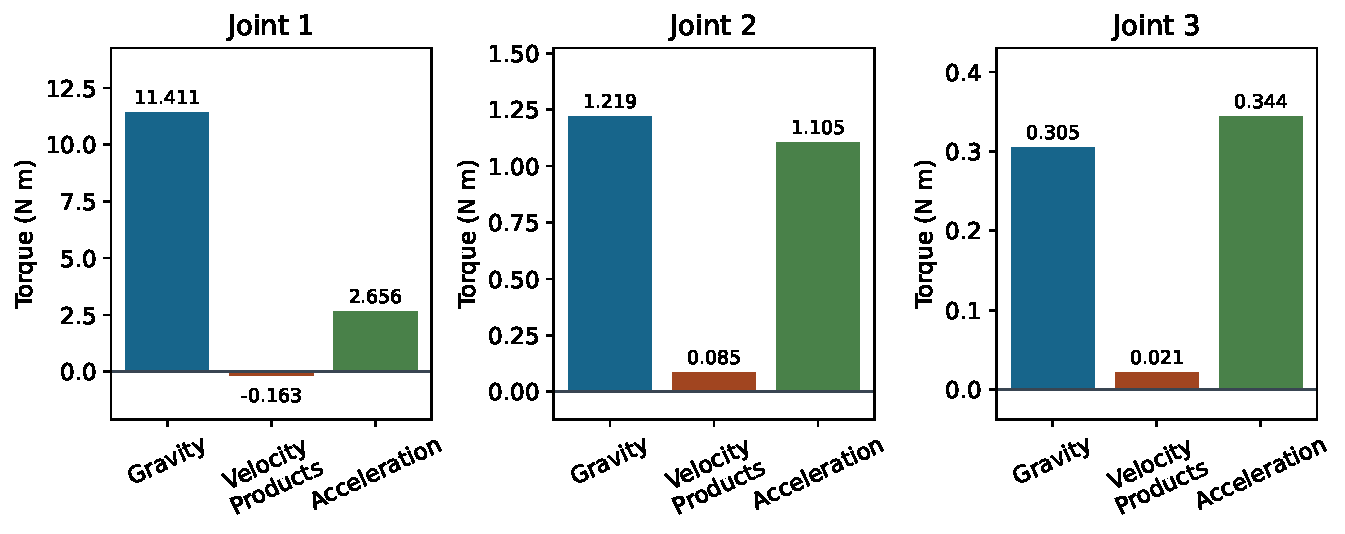
\includegraphics[width=\linewidth]{../figures/recursive_torque.pdf}
\caption{Required Torque Components for the Specified Planar Example. Signed Contributions Depend on the Chosen Pose, Rates, and Accelerations; Each Joint Uses Its Own Torque Scale.}
\label{fig:recursive_torque}
\end{figure}

\section{Validation With Two Uniform Rods}
\label{sec:validation}

Use two rods of unit length and unit mass, with centers halfway along each rod and central planar moments $1/12\,\mathrm{kg\,m^2}$. Keep the same horizontal-zero angle and upward-$y$ gravity convention. The first center is $e_1/2$ and the second is $e_1+e_{12}/2$, where $e_{12}=(\cos(q_1+q_2),\sin(q_1+q_2))$. Differentiating these positions and adding rotational kinetic energy yields
\begin{equation}
 M(q)=\begin{bmatrix}
 5/3+\cos q_2&1/3+\tfrac12\cos q_2\\
 1/3+\tfrac12\cos q_2&1/3
 \end{bmatrix}\,\mathrm{kg\,m^2}.
 \label{eq:rnea_two_rod_mass}
\end{equation}

The potential is $U=g[\tfrac32\sin q_1+\tfrac12\sin(q_1+q_2)]$ in SI units. The velocity-product and gravitational generalized forces are
\begin{equation}
 \begin{aligned}
 b_v&=\tfrac12\sin q_2
 \begin{bmatrix}-2\dot q_1\dot q_2-\dot q_2^2\\\dot q_1^2\end{bmatrix},\\
 G&=g\begin{bmatrix}\tfrac32\cos q_1+\tfrac12\cos(q_1+q_2)\\
 \tfrac12\cos(q_1+q_2)\end{bmatrix}.
 \end{aligned}
 \label{eq:rnea_two_rod_bias}
\end{equation}

The numerical coefficients in $b_v$ carry the unit-rod inertia factors, and those in $G$ carry mass times length. For other dimensions, restore the physical $m,L,c,I_C$ factors before using the formulas. The two-link mass matrix is not obtained by treating each rod as a point mass or omitting its central inertia.

At $q=(0,0)$, $\dot q=(1,0.5)\,\mathrm{s^{-1}}$ and $\ddot q=(0.5,0.2)\,\mathrm{s^{-2}}$, the velocity-product generalized force happens to vanish. The gravity torques are $(19.62,4.905)\,\mathrm{N\,m}$, the acceleration torques are $(1.5,0.483333)\,\mathrm{N\,m}$, and the required torques are $(21.12,5.388333)\,\mathrm{N\,m}$. Vanishing net generalized velocity-product force at this pose does not imply that every local centripetal or spatial-bias term vanishes. Tests at nonzero relative angles are necessary to expose those terms.

\section{The Adjoint From Lie-Group Geometry}
\label{sec:adjoint_derivation}

The same frame law follows by differentiating group conjugation. For a twist matrix $\widehat\xi$, a fixed rigid transform satisfies
\begin{equation}
 T\exp(t\widehat\xi)T^{-1}
 =\exp(tT\widehat\xi T^{-1}),\qquad
 (\operatorname{Ad}_T\xi)^{\wedge}=T\widehat\xi T^{-1}.
 \label{eq:rnea_adjoint_conjugation}
\end{equation}

Conjugation acts on the group; its derivative at the identity acts on the Lie algebra. Composition immediately gives $\operatorname{Ad}_{T_1T_2}=\operatorname{Ad}_{T_1}\operatorname{Ad}_{T_2}$. This makes successive frame changes agree with a single composed change, an important numerical consistency check.

For the differential of the matrix exponential, the noncommutative formula is
\begin{equation}
 D\exp_A[H]=\int_0^1e^{(1-s)A}He^{sA}\,ds.
 \label{eq:rnea_dexp}
\end{equation}

With $A=\widehat\xi$, $H=\widehat\eta$ and $T=\exp(\widehat\xi)$, define the right- and left-trivialized increments explicitly:
\begin{equation}
 \begin{aligned}
 (\delta T\,T^{-1})^{\vee}
 &=\int_0^1\operatorname{Ad}_{\exp(s\widehat\xi)}\eta\,ds,\\
 (T^{-1}\delta T)^{\vee}
 &=\int_0^1\operatorname{Ad}_{\exp(-s\widehat\xi)}\eta\,ds.
 \end{aligned}
 \label{eq:rnea_dexp_trivialization}
\end{equation}

These operators are often named left and right Jacobians according to perturbation conventions; the multiplication order above removes that naming ambiguity. They equal the identity at $\xi=0$. The differential can lose rank at particular exponential-coordinate values even though $T$ and $\operatorname{Ad}_T$ remain invertible. Do not confuse coordinate-chart behavior, a physical task-Jacobian singularity and a rigid frame transformation.

\section{Reproducible Python Examples}
\label{sec:python_rnea}

Run the following from the repository root with its Python dependencies. The first calculation uses the dedicated planar recursion, which permits the endpoint point mass. The second uses the shared spatial-tree RNEA and ABA on three uniform solid cylinders with radius $0.025\,\mathrm m$. These are different mass distributions and therefore have different torques. The spatial example checks a forward/inverse round trip; the analytic two-rod and Cartesian-energy tests supply independent validation rather than relying on that round trip alone.

\clearpage
\begin{lstlisting}[language=Python,basicstyle=\ttfamily\small]
import numpy as np
from scripts.generate_worked_examples import (
    VOL0_CH07_CHAIN, VOL0_CH07_Q,
    VOL0_CH07_QD, VOL0_CH07_QDD,
)
from src.tools.articulated_body_examples import (
    DynamicsLoads, forward_dynamics, inverse_dynamics,
)
from src.tools.articulated_chain_examples import cylinder_chain

q, velocity, acceleration = VOL0_CH07_Q, VOL0_CH07_QD, VOL0_CH07_QDD
recursive = VOL0_CH07_CHAIN.inverse_dynamics(q, velocity, acceleration)
lagrangian = VOL0_CH07_CHAIN.inverse_dynamics_lagrangian(
    q, velocity, acceleration,
)
print("Planar torques:", recursive)
np.testing.assert_allclose(recursive, lagrangian, atol=1e-8, rtol=0)

tree = cylinder_chain(
    np.array([1., .8, .6]), np.array([1., .5, .2]), q, .025,
)
loads = DynamicsLoads(velocity, np.zeros(3))
torque = inverse_dynamics(tree, loads, acceleration)
recovered = forward_dynamics(tree, DynamicsLoads(velocity, torque))
print("Cylinder torques:", torque)
np.testing.assert_allclose(
    recovered.joint_acceleration, acceleration, atol=1e-11, rtol=0,
)
\end{lstlisting}

The cylinder torques for these inputs are approximately
\begin{equation}
 \tau_{\rm cylinder}=(13.447676,1.977061,0.315835)^T\,\mathrm{N\,m}.
 \label{eq:rnea_cylinder_torques}
\end{equation}
 The helper builds transforms that map parent motion into child coordinates and positive-definite cylindrical inertias. Its parent array uses zero-based Python indexing and $-1$ for the base. It accepts constant local one-degree-of-freedom subspaces, known body-frame external loads, uniform gravity, nonnegative diagonal damping and ideal armature. It does not solve contact, floating-base motion, closed loops or flexible-shaft dynamics. Array shape and inertia checks do not prove that an arbitrary supplied transform or inertia is a physically valid model; those remain explicit preconditions.

\section{Interpreting a Golf or Humanoid Model}
\label{sec:ch7_summary}

The outward and inward recursions describe two sides of one coupled mechanism. Geometry determines each joint's motion direction, each point's lever arm and the frame transformations. Mass distribution turns the resulting body velocities and accelerations into momentum and required wrench. The inward pass combines every downstream load, so proximal effort depends on what the distal bodies are doing. Conversely, in forward dynamics, a torque at one joint can accelerate several joints through the coupled inertia and constraints. A temporal sequence of segment-speed peaks alone does not identify which term caused the next peak.

For the club considered as a separate system, hand and shaft-interface wrenches are external loads whose power changes the club's mechanical energy, alongside gravity and other modeled effects. For golfer and club considered together, the paired interface contributions are internal; relative deformation or motion determines whether their summed power transfers, stores or dissipates energy. An ideal stationary ground contact may exchange momentum through force while doing zero power at a nonmoving contact point. Large ground reaction, large joint torque and large positive mechanical work are therefore different observations. A causal argument must state the system boundary, the power pair and the measured or modeled motion.

Joint-space inverse dynamics estimates net mechanical requirements once motion, inertia and external loads are supplied. It does not separate agonist and antagonist muscle forces or determine activation from torque alone. Biarticular muscles distribute forces across joints; activation history and tendon storage can change what torques are feasible at the same mechanical state. Measurement differentiation also amplifies noise, especially in acceleration, so report filtering, uncertainty, synchronization and sensitivity to segment inertias and contact forces.

To investigate a proposed swing mechanism, first reproduce a measured or otherwise specified trajectory within the model's uncertainty. Then define an intervention: alter a particular actuator input, initial state, grip constraint or inertial parameter while stating what is held fixed. Use constrained forward dynamics to calculate the resulting trajectory, and evaluate delivery quantities at the relevant impact event. An instantaneous torque decomposition is useful evidence about required balance; a finite-horizon intervention is needed to support a claim about an outcome. Both contact-mode changes and impact-time shifts can change that conclusion.

The quality of the argument rests on a chain of checkable statements: coordinate consistency, local balance, constraint and actuator feasibility, numerically converged trajectories, and an output tied to the golf question. Recursive algorithms make that chain economical and inspectable. They do not remove uncertainty in anatomy, sensing, constitutive models or human intent.

\section{Further Reading}
\label{sec:further_reading_ch7}

Featherstone's \textit{Rigid Body Dynamics Algorithms} develops spatial inertia and tree algorithms; the author's accompanying coordinate-transform notes distinguish motion and force directions explicitly~\cite{Featherstone2008,FeatherstoneSpatialReview}. Lynch and Park's \textit{Modern Robotics}, Chapter 8, provides a complementary body-twist derivation and separates inverse dynamics from simulation~\cite{Lynch2017}. When consulting code, check whether an external wrench is applied to the body or by the end effector, and whether it is expressed in body or base coordinates. Correct implementations can differ in these conventions.

The following articulated-body chapter develops acceleration elimination and recovery for forward dynamics. Together with the state-space, configuration-space and Lagrangian chapters, it supplies the mechanical basis for later work on control, sensitivity and constrained delivery. A chosen simulator's documentation should supplement these mathematical references with its actual joint, contact, actuation and integration assumptions.

\section{Exercises}

\subsection{Tier 1: Foundations}
\begin{enumerate}[itemsep=3pt,topsep=4pt]
\item \textbf{Invertible Frame Changes.} Derive the inverse adjoint from $T^{-1}$. Show directly that a pure translation gives an invertible motion transform, even though its angular screw component is zero.
\item \textbf{Tree and Joint Conventions.} Give the one-based parent array for a two-link planar chain with base 0. Write its local revolute subspaces at the proximal origins and the relative motion transforms for horizontal-zero angles. Explain how the Python indexing differs.
\item \textbf{A Nonzero Planar Bracket.} For angular-first $V=(\omega,v)$, take $\omega=(0,0,0.5)$ and $v=(0.4,0,0)$. A revolute joint at the origin about local $+z$ has rate $\dot q=0.2$. Calculate all six components of $\operatorname{ad}_VV_J$. Identify the physical units of the nonzero component and explain why an angular-only cross product misses it.
\item \textbf{Power and Wrench Direction.} Starting from $V_A=X_{AB}V_B$, derive both force transformation directions. Use a translated origin and a nonzero force to show why inverse-transpose child-to-parent propagation would give the wrong moment.
\item \textbf{Inertia and Degeneracy.} Construct the planar inertias of the three-link example from its masses, center offsets and central moments. Explain why its endpoint point mass is compatible with a nonsingular restricted joint-space mass matrix but does not have a positive-definite six-dimensional spatial inertia.
\end{enumerate}

\subsection{Tier 2: Mechanics and Verification}
\begin{enumerate}[itemsep=3pt,topsep=4pt]
\item \textbf{Newton--Euler From Energy and Momentum.} Derive the center-of-mass force and moment equations, including the gyroscopic term, and transform them to a noncentral origin. Use virtual power to explain their equivalence to the generalized Lagrangian equations.
\item \textbf{A Genuine Branch.} For parents $(0,1,1,3)$, write the complete inward accumulation, including a known external load on body 1 and on both leaves. Identify which body efforts are influenced by each leaf load.
\item \textbf{Dual Operators.} Verify $V\times^*=-\operatorname{ad}_V^T$ numerically. Check preservation of power under a nontrivial rotation and translation, then compare the two uniform-rod torques with the closed forms at three nonsymmetric configurations.
\item \textbf{Like-for-Like Computational Comparisons.} For $N=5,10,20,50$, compare RNEA with a preassembled $M\ddot q+h$ evaluation as inverse-dynamics tasks. Separately compare ABA with a mass-matrix forward solve. Report model preparation, factorization reuse, hardware, repetitions and numerical agreement; distinguish expected arithmetic growth from measured timing.
\item \textbf{A Cut Loop.} Introduce a bilateral closure constraint into an otherwise open tree. Derive the acceleration constraint and coupled force solve. State what changes if the constraint rows are redundant or the prescribed inverse-dynamics motion is inconsistent.
\end{enumerate}

\subsection{Tier 3: Modeling and Extension}
\begin{enumerate}[itemsep=3pt,topsep=4pt]
\item \textbf{Composition.} Prove the adjoint homomorphism using group conjugation and verify it with two translated, rotated frames. Show that the corresponding force transforms preserve the same composition order in the same direction.
\item \textbf{Differentiating the Exponential.} Derive the integral formula for $D\exp_A[H]$, then both explicitly ordered trivializations. Compare with centered finite differences for noncommuting $A,H$ and explain why $e^AH$ is insufficient in general.
\item \textbf{A Declared Humanoid Tree.} Specify a teaching humanoid with 30 independent velocity degrees of freedom, stating whether six belong to a floating base. Provide a parent structure, joint types, axes, body inertias, actuation map and contact assumptions. Explain which accelerations can be prescribed consistently and which base-force equations remain unactuated.
\item \textbf{Composite Versus Repeated Inverse Dynamics.} Implement composite-inertia accumulation and ancestor projection to form $M$. Compare it with the bias-subtracted RNEA columns and the kinetic-energy construction. Separate the linear composite pass from worst-case quadratic full-matrix output, and identify the zero couplings between independent branches of a fixed-base tree.
\item \textbf{Compliant Contact and Delivery.} Add a specified nonadhesive compliant contact law to a simple forward-dynamics model. Perform timestep refinement and check contact work and force convergence. Explain how stiffness, damping, effective mass, actuator limits and an event-defined delivery output interact; do not infer numerical stability from the force law alone.
\end{enumerate}
